\section{Protection of Air-sensitive Samples for Electric Measurement}
\label{sec:expsetup:airsensitive}

The Dirac semimetal Na$_3$Bi is an air-sensitive crystal. Due to the chemical reactivity of sodium, the whole Na$_3$Bi crystal can be easily oxidized in the air within ten seconds. Therefore, we need to make contacts to the sample within the glove box and then seal it well. The sample can only be loaded into the cryostat when it's isolated from any air or water. Great care should be taken during the process. Any remnant oxygen or water in the glove box, or any leaks in the seal can easily turn the crystal into ashes. 

Such fragileness of Na$_3$Bi crystals has created a large obstacle for us to make the electric contacts. To avoid any oxidization, we have to make contacts to the sample in the Argon glove box. Here we use silver epoxy (Epotek H20E) to fix the platinum wires on the crystals. We first put Pt wires and the silver epoxy on the right spot of the samle, then heat it at around 120 $\celsius$ for about 5 minutes so that the silver epoxy matures. Then we put the sample inside a small cylinder container as shown in Fig. \ref{Na3Bi_container} and connect the Pt wires to the electric pads on the cap of the container. We diminish the chance of oxidization by adding paratone oil inside the container after the sample is mounted. Thus the sample is completely immersed in the paratone oil. Then the container is sealed and put into a cryostat for the measurement. Our results show that the sample can survive inside the container for a couple of days even when the container is exposed to air. Once the crystal is loaded into a cryostat and stays below 100 K, the sample stays the same during a long time of measurement. Hence we are able to measure the same Na$_3$Bi sample in different cryostats for a long time.


\begin{figure}[!htbp]
  \begin{center}
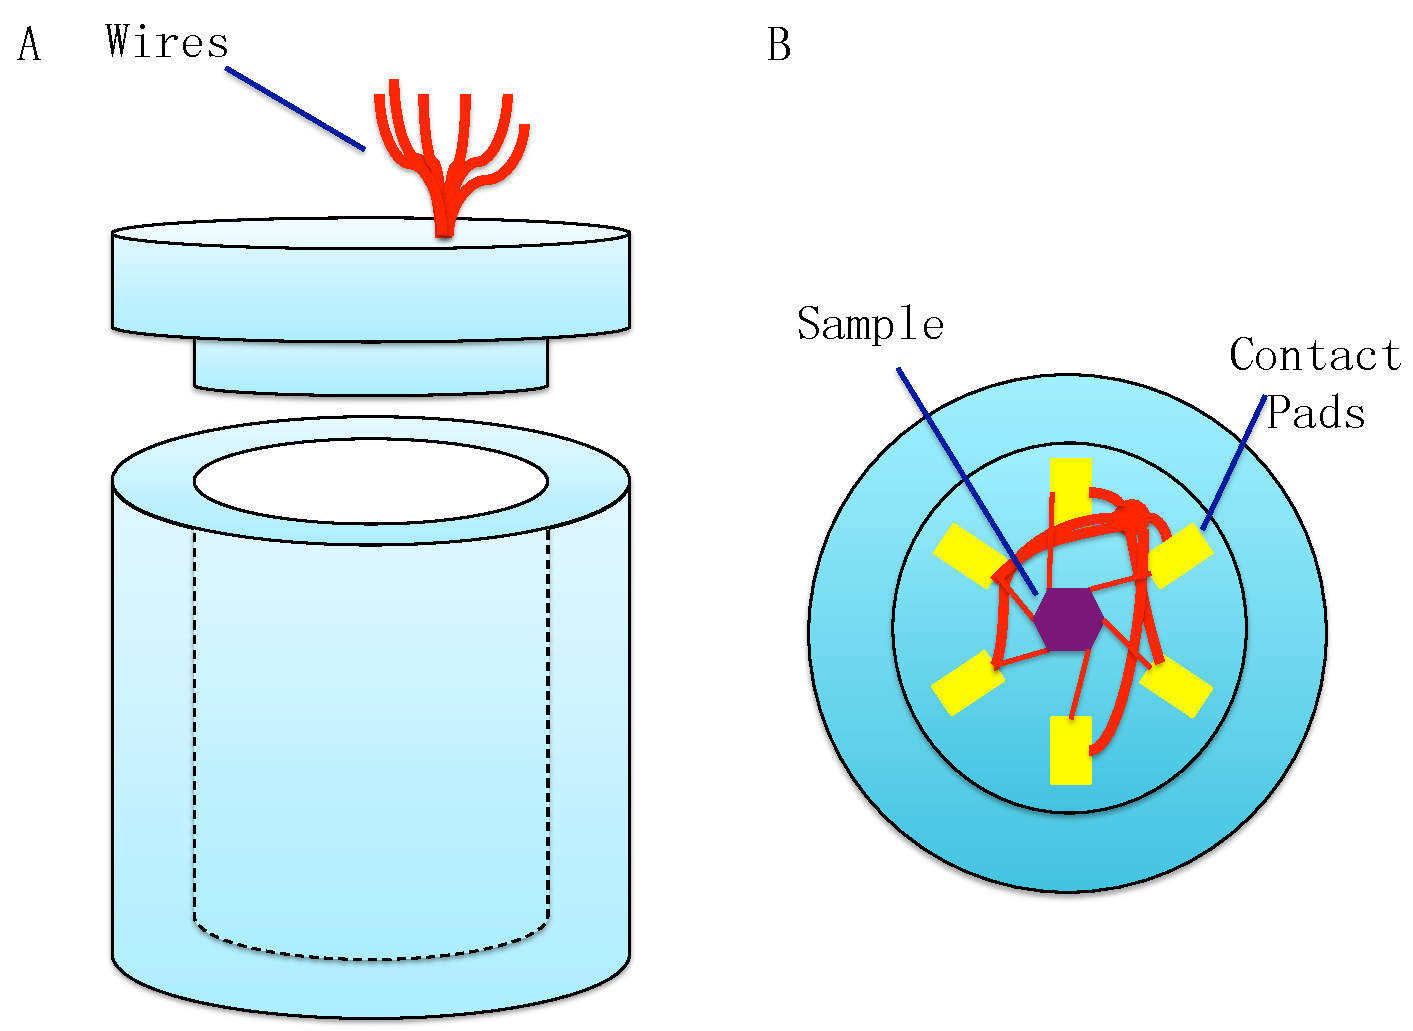
\includegraphics[width=0.8\linewidth]{ch-expsetup/figures/Na3Bi_container.pdf}
\caption{\label{Na3Bi_container}
A sketch of the container that we use to protect the Na$_3$Bi crystal. Panel (A) shows that the container has a bucket and a cap. There are wires  going through the cap. Before the seal, the main bucket is filled with paratone oil to prevent oxidization. Panel (B) shows that the sample is mounted on the inner side of the cap. There are Pt wires connecting the sample and the contact pads on the cap. 
}
  \end{center}
\end{figure}





